\chapter{String Regeneration Applied to Machine Translation}
\chaptermark{String Regeneration for Translation}
\label{chap:gyroTrans}

% TODOFINAL crowdflower eval
% TODOFINAL grep bag-of-word and add s where needed
% TODOFINAL review preamble and correct pdfinfo
% TODOFINAL grep for chunk and maybe rephrase
% TODOFINAL grep for lmbr and harmonize capitalization
% TODOFINAL grep for data and replace by text where appropriate
% TODOFINAL grep for stupid and put capital S
% TODOFINAL grep for CUED and Cambridge University Engineering Department
% TODOFINAL harmonize notation for NIST openMT etc.
% TODOFINAL grep for config and replace with configuration
% TODOFINAL harmonize notation 1st pass vs. first pass first-pass
% TODOSUBMIT remove mismatch between 34.92 and 34.96
% TODOFINAL add row numbers to all tables
% TODOFINAL replace 1-best by 1st-best where appropriate
% TODOFINAL (done ?) make short running title

In \autoref{chap:gyro}, we have introduced
techniques for string regeneration inspired from
the phrase-based translation paradigm.
We have demonstrated their effectiveness
and achieved state-of-the-art performance in terms of
BLEU on the string regeneration task on the Penn Treebank.
In this chapter, we will attempt to apply these techniques to the output
of a machine translation system. One key difference is that
the quality of the input bag of words is substantially lower when
regenerating translation output instead of regenerating
an original English sentence.

Our motivation is the general motivation for the rescoring paradigm.
Instead of allowing any kind of reordering in first pass
decoding, which would make the search space intractable, we first create a
search space of relatively high
quality, then we relax reordering constraints.
We will show that using our string regeneration decoder,
we are able to match the quality of our translation
system. In some instances, we show very slight gains in
performance. This work is meant to lay the ground
work for future incorporation of natural language
generation into SMT.

In \autoref{sec:gyroTransExpSetting}, we describe
our machine translation baseline system.
In \autoref{sec:gyroTransBaseline}, we describe
our string regeneration baseline, both with and without
future cost estimates. Because the regeneration baseline
degrades performance with respect to the translation
baseline, we carry out an error analysis
in \autoref{sec:gyroTransErrorAnalysis}.
In \autoref{sec:gyroTransBiasedLm} and
in \autoref{sec:gyroTransSysComb}, we show two ways of incorporating
information from the translation system in order to match
the translation system quality; in some instances,
we obtain very slight improvements over the MT baseline.
%Finally, in \autoref{sec:gyroTransConfidenceRegions} (TODONEVER section being written
%because still waiting for results), we show
%how to exploit confidence regions in
%the translation system lattice output in order to segment
%the translation output in a meaningful way prior to running
%our regeneration decoder.

\section{SMT Baseline System}
\label{sec:gyroTransExpSetting}

In this section, we briefly summarize the machine translation
system used as a baseline for our string regeneration rescoring
experiments.
%
%chinese wc: 9221421 202984470 764720109
%english wc: 9221421 218009927 766246848
%
The Cambridge University Engineering Department participated in the
NIST 2012 translation
competition.\footnote{\url{http://www.nist.gov/itl/iad/mig/openmt12.cfm}}
We describe here the Chinese-English system. We pick this language
pair rather than for example Arabic-English simply because Chinese
and English are quite distant in terms of word ordering (see \autoref{sec:hierintro}).

We use all the Chinese-English parallel data
available for the constrained track. Parallel data consists
of 9.2M sentence pairs, 203M tokens on the Chinese side and
218M tokens on the English side, after preprocessing.
Parallel data is aligned using a word-to-phrase
HMM model with the MTTK
toolkit (see \autoref{sec:statisticalMachineTranslationHmmAlignmentModel}).
In the source-to-target direction, the maximum size of a Chinese phrase is 2 while
in the target-to-source direction, the maximum size of an English phrase is 4. % TODOFINAL ask Bill for confirmation and/or any justification (citation ?)
The final alignments are obtained by taking
the union of Viterbi alignments obtained
in both source-to-target and target-to-source directions.
A hierarchical phrase-based grammar is then extracted from
the alignments using the infrastructure described
in \autoref{sec:rulextractMapReduce}.

We build a first-pass language model using the target side
of the parallel text and the AFP and Xinhua agencies of the
GigaWord~\citep{parker-graff-kong-chen-maeda:2009:LDC}. % TODOSUBMIT review bibtex entry
We first build separate modified Kneser-Ney smoothed 4-gram language
models (see \autoref{sec:StatisticalMachineTranslationKneserNey})
on each of these three corpora. The language models built on AFP
and Xinhua are interpolated with equal weights. The
resulting language model is interpolated with the
language model built on the target side of the parallel
text with equal weights. We also build a second-pass % TODOFINAL explanation that this is not the best strategy (see WMT chapter). but it doesn't matter for this anyway.
Stupid Backoff 5-gram language model for rescoring
as described in \autoref{sec:rescoring}.
The output of 5-gram rescoring is rescored with LMBR (see \autoref{sec:lmbr}).

We use the features described in \autoref{sec:features}
as well as 36 provenance related features (see \autoref{sec:domainAdaptationGrammar}).
The union
strategy is employed for test set grammar filtering, as described
in \autoref{sec:domainAdaptationGrammar}.
In this chapter, all results are reported on an internal tuning set (Tune)
in the newswire domain comprising
1755 sentences and on the newswire portion of the NIST
2008\footnote{\url{http://www.itl.nist.gov/iad/mig/tests/mt/2008/}} test
set comprising 691 sentences (MT08).

The results are reported in \autoref{tab:nist12results}.
For information, the system submitted for the NIST12 evaluation was based
on hypothesis combination over various preprocessing of the source and obtained
a score of 33.90 BLEU on the newswire portion of the MT12 test set.
%
\begin{table}
  \begin{center}
    \begin{tabular}{l|lll}
      Configuration   & Tune & MT08 \\
      \hline
      MT baseline 1st pass & 34.92 & 35.71 \\
      MT baseline +5g      & 36.04 & 36.60 \\
      MT baseline +lmbr    & 36.80 & 37.59 \\
    \end{tabular}
    \caption{CUED NIST 2012 system performance as measured by case insensitive BLEU on MT08. The output of the
      first pass decoder will serve as input to the regeneration decoder.}
    \label{tab:nist12results}
  \end{center}
\end{table}

In the next section, we will describe our string regeneration setting where
the output of the translation system is taken as input by our
regeneration decoder.

\section[Regeneration Decoder Baseline on MT Output]{Regeneration Decoder Baseline \\ on MT Output}
\label{sec:gyroTransBaseline}

% TODOFINAL check NgramGen naming (vs. gyro and capitalization also)

In this section, we describe how the first-pass output
of the SMT system described in \autoref{sec:gyroTransExpSetting}
is processed as input by the NgramGen regeneration decoder.
We consider a test set with $N$ source sentences
$\bm{f_1}$, ..., $\bm{f_N}$ to be translated.
The first-pass translation decoder generates $N$ sets of hypotheses % VIVA Q: why first pass A: so we can apply rescoring
encoded as $N$ lattices $\mathcal{H}_1$, ..., $\mathcal{H}_N$.
We extract 10-best lists from these lattices.
The $i$-th-best translations are denoted $\bm{e}_1^i$, ..., $\bm{e}_N^i$.
Thus we obtain
10 sets of bags-of-words. The first set of bags-of-words consists
of the best first-pass translations for each source sentence, that is
$\bm{e}_1^1$, ..., $\bm{e}_N^1$, and so on
for the second set up to the tenth set of bags, which contains
$\bm{e}_1^{10}$, ..., $\bm{e}_N^{10}$. Clearly, the quality of
bags-of-words decreases as we go from the first set of bags to the
tenth set.

We then run our regeneration decoder
NgramGen on each
set of bags-of-words separately. The configuration for running
the decoder on the $i$-th set of bags is called $i$th-best.
We obtain
$N$ lattices $\mathcal{L}_1^1$, ..., $\mathcal{L}_N^1$ for the first set of bags,
and so on for the second set of bags to the tenth set of bags, for which we
obtain $N$ lattices $\mathcal{L}_1^{10}$, ..., $\mathcal{L}_N^{10}$.
Performance is measured
on each separate set of NgramGen output lattices.
Intuitively, we can predict that the performance will decrease from
the NgramGen output for the first set of bags to the NgramGen output for
the tenth set of bags.

We also form the union of lattices
obtained from each set:
for the i-th source sentence $\bm{f_i}$, we form the union
of the lattices $\mathcal{L}_i^1$, ..., $\mathcal{L}_i^{10}$.
This configuration is simply
called \emph{union}.
We use the following settings for the regeneration decoder:
%
\begin{itemize}
  \item We use a histogram pruning of 1000, that is a maximum number of 1000 states
    per column (see \autoref{sec:gyroPruningDescription}).
  \item We split the input according to punctuation (comma and semi-colon), with
    a maximum chunk length of 11, as described in \autoref{sec:sentenceSplitting}.
    Note that contrary to the string regeneration settings, the splitting information
    comes from an MT hypothesis and not a reference. Therefore, it is legitimate
    to use input splitting for experimentation, decoding times become more
    reasonable and the NgramGen hypotheses are constrained to be close to
    the MT hypotheses, which we know have a relatively high quality already.
  \item As in \autoref{sec:gyroFutureCost}, future cost is estimated with a unigram language model.
\end{itemize}
%
Results are summarized in \autoref{tab:gyroMTbaseline}.
The main observation is that for all regeneration configurations, there
is a substantial drop in performance with respect
to the machine translation baseline. This is not unexpected
since we are only using the language model feature for regeneration:
except for the bag-of-words obtained from the translation hypothesis and
the splitting points for more efficient decoding, all information coming from the translation system
is discarded.

We measured the performance of the oracle hypothesis % TODOFINAL explain how to obtain that and refer to background
for the translation system and the regeneration systems on the Tune set.
Again, regeneration oracle BLEU scores are substantially
lower than the translation oracle BLEU.
However, it interesting to observe that
the oracle hypothesis obtained from the union configuration is
around 9 BLEU points above the MT baseline. This indicates that
there is a possible reordering of the 10-best hypotheses obtained by
the translation decoder that improves translation quality.

Experiments were run with and without future cost estimates.
We obtain small gains when future cost estimates are used (see column 3 vs.\ column1,
column vs.\ column 2 and column 6 vs.\ column 5)
but gains are very small compared to what was obtained
when regenerating a well-formed English sentence as in \autoref{sec:gyroFutureCost}.

Finally, as predicted, because the quality of the bags decreases from the 1st-best configuration
to the 10th-best configuration, performance after regeneration from these sets of bags also decreases.
In the next section, we will analyze the drop in performance
for the regeneration configuration with respect to the MT
baseline.
%
\begin{table}
  \begin{center}
    \begin{tabular}{l|l|l|l|l|l|l}
      Column        & 1    & 2    & 3    & 4    & 5     & 6 \\
      \hline
      Set & Tune & Tune & Tune & Tune &  MT08 & MT08 \\
      \hline
      Oracle        &      & \Checkmark & & \Checkmark & & \\
      \hline
      MT baseline 1st pass & 34.96 & 56.12 & 34.96 & 56.12 & 35.71 & 35.71 \\
      \hline
      Future Cost &         &           & \Checkmark & \Checkmark & & \Checkmark \\
      \hline
      1st-best & 33.37 & 39.14 & 33.40 & 39.18 & 32.78 & 32.79 \\
      2nd-best & 33.16 & 38.93 & 33.22 & 39.02 & 32.77 & 32.77 \\
      3rd-best & 33.14 & 38.84 & 33.17 & 38.91 & 32.54 & 32.55 \\
      4th-best & 33.13 & 38.80 & 33.16 & 38.87 & 32.35 & 32.39 \\
      5th-best & 33.20 & 38.95 & 33.28 & 39.00 & 32.12 & 32.17 \\
      6th-best & 33.08 & 38.74 & 33.12 & 38.81 & 32.33 & 32.40 \\
      7th-best & 33.19 & 39.00 & 33.24 & 39.05 & 32.16 & 32.18 \\
      8th-best & 32.98 & 38.79 & 33.04 & 38.84 & 32.11 & 32.14 \\
      9th-best & 32.71 & 38.59 & 32.75 & 38.65 & 32.11 & 32.11 \\
      10th-best & 33.05 & 38.81 & 33.11 & 38.88 & 32.50 & 32.55 \\
      \hline
      union & 32.85 & 43.96 & 32.90 & 44.00 & 32.11 & 32.18 \\
    \end{tabular}
  \end{center}
  \caption{Regeneration experiments on input bags obtained from the
    10-best hypotheses of a translation system. Case-insensitive BLEU
    scores are reported. 10-best lists are generated by an MT system.
    Each set of $n$th-best hypotheses is used as a set of input bags-of-words
    for the NgramGen decoder. Oracle performance on the Tune set is also measured.
    Regeneration decoding experiments are repeated with and without future cost estimates.
    Substantial drops in performance are observed in regeneration with respect to the
    translation baseline. Oracle scores for the union configuration show that
    by simply improving word reordering on the 10-best output of the MT system, gains may
    be achieved. Future cost estimates provide very small gains.}
  \label{tab:gyroMTbaseline}
\end{table}
%

\section{Analysis of the Loss of MT Hypotheses}
\label{sec:gyroTransErrorAnalysis}

% TODOFINAL maybe compare lm costs

We have observed in the previous section that simply reordering the $n$-best output
of the translation decoder with our regeneration decoder gives a drop
in performance with respect to the performance obtained by the
baseline translation system.
Although the translation system output lacks fluency due to word reordering
problems, we know that the quality of this output is relatively high, thus
we would like the output of the regeneration step to stay relatively close
to the MT hypothesis.
In this section, we will examine how often the MT
hypothesis is not regenerated at all in the regeneration lattices, how often it is
chosen as a regeneration hypothesis and at what point in the decoding procedure
the MT hypothesis disappears from the regeneration lattice.
We carry out this analysis on the 1st-best configuration from
\autoref{tab:gyroMTbaseline} and on the Tune set.

The MT hypothesis is present in the regeneration lattice
92.3\% of the time when no future cost is estimated and
95.3\% of the time with future cost estimates. This is somewhat reassuring
because these numbers imply that the language model score of the MT
hypothesis is high enough so that the MT hypothesis is not very frequently discarded
by pruning in regeneration.
In contrast, the MT hypothesis is chosen as the
best hypothesis by the regeneration decoder only 43.6\% of the time, with
or without future costs. This means that, most of the time, the MT
hypothesis is present in the regeneration lattice, but not chosen as
the best regeneration hypothesis, simply because its model score, computed
by the language model only, is lower than the score of another
regeneration hypothesis.

For the case when the MT hypothesis is not present in the regeneration
lattice, we further analyze at which point the MT hypothesis is lost
during the decoding procedure. As described in \autoref{sec:gyroStateDefinition},
a state is defined by coverage and history. For this analysis, we
add a Boolean variable to the state definition that indicates whether
the partial input is one of the partial hypotheses represented by this state.
We can then easily compute after how many words covered the MT hypothesis
has been lost.

\autoref{fig:whenLostInput} illustrates the proportion of MT hypotheses
lost vs.\ the proportion of input words covered.
The plot shows that
MT hypotheses can be lost quite early in the process, as early as
when 20\% of the size of the input bag-of-word has been covered.
Using future cost estimates produces a very similar graph and does not
alleviate the problem of losing MT hypotheses early in the decoding process.
%
\begin{figure}
\begin{center}
%\begin{minipage}{.45\textwidth}
  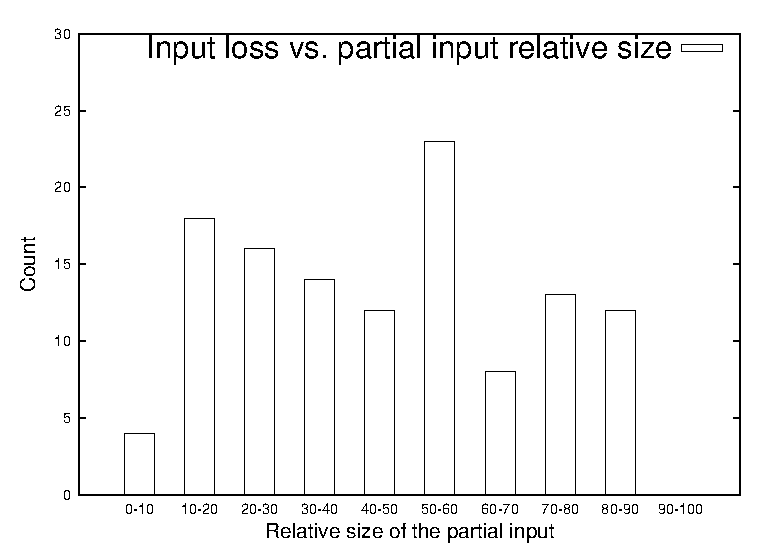
\includegraphics[scale = 0.8]{figures/whenLostInput/Tune.text.nw.v3x08.1stpass.10best.exp.allrules.mmap.nbest1000.1.whenlostinput.eps}
%\end{minipage} 
%\hfill
%\begin{minipage}{.45\textwidth}
%  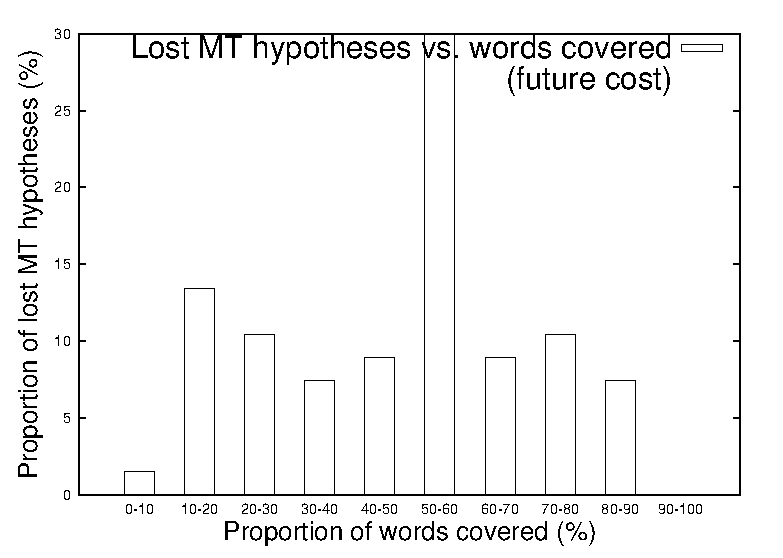
\includegraphics[scale = 0.6]{figures/whenLostInput/Tune.text.nw.v3x08.1stpass.10best.exp.allrules.mmap.nbest1000.1.futurecost.whenlostinput.eps}
%\end{minipage}
\caption{Analysis of when the MT hypothesis is lost. The x-axis represents bins of 10\% for the relative size of the input bag-of-word.
The y-axis is simply the count of instances.}
\label{fig:whenLostInput}
\end{center}
\end{figure}
%

From this analysis, we conclude that using the language model score as
a single feature is not adequate for the task of regeneration from
translation output. Designing and implementing additional features is
a worthwhile opportunity for future work. In the sections to follow, while
keeping a single feature for regeneration, we will study
alternative ways to bring the regeneration output closer to the translation output.

\section{Biased Language Model for Regeneration}
\label{sec:gyroTransBiasedLm}

We have shown in \autoref{sec:gyroTransErrorAnalysis} that the MT
hypothesis, which is known to
be of relatively high quality, is not chosen as the best regeneration
hypothesis more than half of the time and is sometimes not even
present in the regeneration lattice.
In this section, we describe a first solution to remedy this issue and
bring the regeneration output closer to the translation output.

Our solution is simply to bias the language model towards the MT hypothesis.
In order to do this, we first compute $n$-gram posterior probabilities
from the
1st-pass translation lattices (see \autoref{sec:lmbr}).
These posteriors are then converted
to integer counts in order to estimate a
Good-Turing~\citep{good:1953:biometrika,chen-goodman:1998:harvard} smoothed 4-gram % TODOFINAL Good-Turing in background
% VIVA Q: why Good-Turing ? A: it's the default in SRILM :)
language model from these counts.
We then interpolate this language model with the original language model with
various interpolation parameters.

We report on experiments that are carried out on the set of bags obtained from the best MT hypotheses;
experiments on lower quality bags gave analogous results.
Interpolation parameters range
from 0.4 (weight assigned to the original language model) to 0.99.
We obtain the results in \autoref{tab:gyroBiasedLm}.
We can see that we are able to obtain hypotheses that have
the same quality as the MT hypotheses, and for an interpolation
weight of 0.7, we obtain a very slight improvement on the tuning
set. We also obtain very similar results when future cost estimates are included.
%
\begin{table}
  \begin{center}
    \begin{tabular}{l|l|l}
      Configuration      & \multicolumn{2}{c}{Tune} \\
      \hline
      MT baseline 1st pass & \multicolumn{2}{c}{34.96} \\
      \hline
      Future Cost &  & \Checkmark \\
      \hline
      1st-best      & 33.37 & 33.40 \\
      \hline
      1st-best 0.4  & 34.96 & 34.95 \\
      1st-best 0.5  & 34.96 & 34.96 \\
      1st-best 0.6  & 34.96 & 34.96 \\
      1st-best 0.7  & 34.97 & 34.96 \\
      1st-best 0.8  & 34.94 & 34.94 \\
      1st-best 0.9  & 34.90 & 34.90 \\
      1st-best 0.95 & 34.81 & 34.81 \\
      1st-best 0.99 & 34.11 & 34.13 \\
    \end{tabular}
    \caption{Regeneration experiments on the set of bags obtained
      from the best MT hypotheses, with biased language models.
      Case-insensitive BLEU scores are reported.
      The original language model is interpolated with a language
      model built from MT posteriors. A range of interpolation
      parameters is experimented on. It is possible to recover
      the MT performance when the interpolation weight for the MT posterior
      based language model is large enough. Including future cost estimates
      gives very similar results.}
    \label{tab:gyroBiasedLm}
  \end{center}
\end{table}
%

We use the best configuration from \autoref{tab:gyroBiasedLm}
(interpolation weight of 0.7) to run
our regeneration decoder on the test set MT08 and obtain the results
in \autoref{tab:gyroBiasedLmTest}.
We obtain slight gains in terms of BLEU score on the MT08 test
using this technique. 
%
\begin{table}
  \begin{center}
    \begin{tabular}{l|l|l}
      Configuration & Tune & MT08 \\
      \hline
      MT baseline 1st pass & 34.96 & 35.71 \\
      \hline
      1st-best 0.7 & 34.97 & 35.75 \\
      1st-best 0.7 future cost & 34.96 & 35.75 \\
    \end{tabular}
    \caption{Regeneration with a language model biased towards MT
      posteriors. Case-insensitive BLEU scores are reported.
      The best configuration from \autoref{tab:gyroBiasedLm} is
      used to carry out regeneration on the MT08 test set. Very slight
      gains are observed.}
    \label{tab:gyroBiasedLmTest}
  \end{center}
\end{table}

% TODOFINAL maybe redo with less pruning ??

%biased lm union
%\begin{table}
%  \begin{center}
%    \begin{tabular}{l|l|l}
%      Config      & BLEU & Oracle BLEU \\
%      MT Baseline & 34.96 & 56.12 \\
%      union       & 0.3285 & 43.96 \\
%      union 0.4   & TODONEVER
%      union 0.5
%      union 0.6
%      union 0.7
%      union 0.8
%      union 0.9
%      union 0.95
%      union 0.99
%    \end{tabular}
%    \caption{caption}
%  \end{center}
%\end{table}

%biased lm future cost
%\begin{table}
%  \begin{center}
%    \begin{tabular}{l|l|l|l}
%      Config      & BLEU & Oracle BLEU & MT08 \\
%      MT Baseline & 34.96 & 56.12 & 35.71  \\
%      1-best      & 33.40 & 39.18 & 32.79 \\
%      1-best 0.4  & 34.95 & & \\
%      1-best 0.5  & 34.96 &  & \\
%      1-best 0.6  & 34.96 &  & \\
%      1-best 0.7  & 34.96 & & 0.3575 YAY! \\
%      1-best 0.8  & 34.94 & & \\
%      1-best 0.9  & 34.90 & & \\
%      1-best 0.95 & 34.81 & & \\
%      1-best 0.99 & 34.13 & & \\
%    \end{tabular}
%    \caption{caption}
%  \end{center}
%\end{table}

\section[Translation and Regeneration Hypothesis Combination]{Translation and Regeneration \\ Hypothesis Combination}
\label{sec:gyroTransSysComb}

% TODOFINAL this transition is too concised, expand

In \autoref{sec:gyroTransBiasedLm}, we have described
a first solution to bringing the quality of regeneration
to the level of translation: biasing the language model using
MT posteriors.
Another possibility is exploit
the system combination paradigm.
Because the regeneration decoder produces FSTs, we can
reuse an existing hypothesis combination system based on FSTs and
described in \autoref{sec:lmbrSysComb}.
Hypothesis combination can also be used in conjunction
with the biased language model presented in \autoref{sec:gyroTransBiasedLm}.

The output of the regeneration decoder is first rescored with
the large 5-gram language model described
in \autoref{sec:gyroTransExpSetting} and then combined with the
5-gram rescored MT hypotheses.
We experiment on the
1-best configuration (the set of bags is obtained
from the best first-pass MT hypotheses) and on the union
configuration (see \autoref{sec:gyroTransBaseline}).
Configurations for the regeneration decoder also
include the baseline reported in \autoref{sec:gyroTransBaseline}
as well as the biased language model method with an interpolation
weight of 0.7 presented in \autoref{sec:gyroTransBiasedLm}.

Results are reported in \autoref{tab:gyroTransSysComb}.
We can observe that using the union of lattices produced
by NgramGen is beneficial for hypothesis combination: more hypotheses
are present in lattices obtained with the union configuration.
Using the biased language model described in the
previous section, we are able to match and obtain
a very slight gain over the LMBR rescored translation
hypotheses.
%TODOFINAL add row numbers
\begin{table}
  \begin{center}
    \begin{tabular}{l|l|l}
      Configuration & Tune & MT08 \\
      \hline
      MT baseline +lmbr & 36.80 & 37.59 \\
      \hline
      NgramGen 1-best baseline &  36.81 & 37.29 \\
      NgramGen union baseline & 36.81 & 37.50 \\
      \hline
      NgramGen 1-best baseline future cost & 36.82 & 37.45 \\
      NgramGen union baseline future cost & 36.81 & 37.50 \\
      \hline
      NgramGen 1-best interpolation 0.7 & 36.82 & 37.39 \\
      NgramGen union interpolation 0.7 & 36.78 & 37.59 \\
      \hline
      NgramGen 1-best interpolation 0.7 Future Cost & 36.81 & 37.39 \\
      NgramGen union interpolation 0.7 Future Cost & 36.77 & \textbf{37.60} \\
    \end{tabular}
    \caption{Experiments in hypothesis combination between the 5-gram rescored
      output of the translation
      decoder and the 5-gram output of the regeneration decoder.}
    \label{tab:gyroTransSysComb}
  \end{center}
\end{table}

%\section{Exploiting Confidence Regions}
%\label{sec:gyroTransConfidenceRegions}

%\begin{table}
%  \begin{center}
%    \begin{tabular}{l|l|l}
%      Config & Tune & MT08 \\
%      MT Baseline & 34.96 & 35.71 \\
%      Gyro Baseline & 33.37 & 32.78 \\
%      beta 0.3 & 32.93 &  \\
%      beta 0.4 & 32.94 & \\
%    \end{tabular}
%    \caption{TODONEVER caption}
%  \end{center}
%\end{table}

\section{Conclusion}

In this chapter, we have demonstrated how to apply our regeneration
decoder to the output of a translation system in a 10-best hypothesis
rescoring setting. Because the regeneration decoder only uses
a language model as single feature and throws away word order
information obtained from the translation system except for splitting
the input bag-of-word, by simply
applying the NgramGen decoder to the output of the translation system, translation
performance is degraded.

We have shown two possible ways of integrating the information from the
translation system into the regeneration system in order to match
and slightly outperform the translation quality obtained by the
translation system. The first solution is to bias the language
model used in regeneration towards the MT hypotheses by building an interpolated
model between the original language model and a language model built on the MT
posteriors. The second
solution simply takes advantage of the hypothesis combination paradigm.
In addition, both solutions were used in conjunction by combining the output
of the MT system with the output of regeneration system where the language model
was biased.

One possible avenue for future work is to design and implement additional
features in the decoder. The use of a few simple features, such as word and rule count, was
already investigated but these features were not found to be beneficial.
Because the regeneration system was introduced into translation with no loss
in performance, another interesting next goal will be to keep identical performance
and use the NgramGen system in order to improve fluency.

%\begin{itemize}
%  \item Experiment with bag of word made of 1-best translation. Show oracle scores. OK
%  \item Experiment with bag of word made of 1-best to 10-best translation. Show oracle scores. OK
%  \item Error analysis: show how often at what stage the input is lost. Conclusion: the
%    decoder needs to be biased towards the input. OK when lost input OK
%  \item Experiments on biasing the decoder towards the input: build language models
%    based on the MT output or based on the MT posteriors. OK
%  \item System combination experiments. OK
%  \item MAYBE: Syntactic n-grams experiments: use the syntactic n-grams to enrich the
%    bag of words and use the dependencies in conjunction with the dependency LM.
%  \item Use gyro together with confidence regions: the confidence regions can be used
%    for chopping and constraints. RUNS
%  \item MAYBE: Use gyro together with position specific posteriors (TBA).
%\end{itemize}
